\chapter{関連技術}
\label{chap:related_works}

本章では,本研究で基盤技術として使用するRDMA(Remote Direct Memory Address),およびlibtlpに関して述べる.

\section{vmを用いた解析}

\subsection{qemu}

\subsection{libvmi}

\section{RDMA}

ここにRDMAの説明をかく

\begin{figure}[htbp]
    \caption{PCI Express}
    \label{fig:zentai}
    \begin{center}
        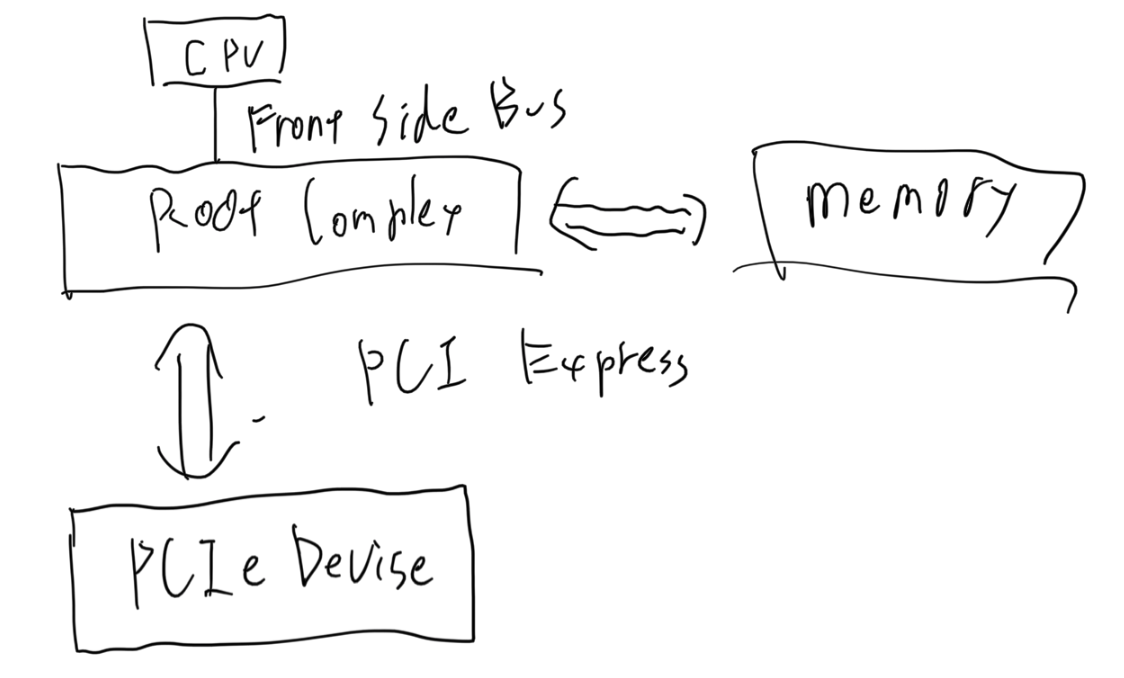
\includegraphics[bb=0 0 1000 400,width=15cm]{img/tegaki/pcie.png}
    \end{center}
\end{figure}

\subsection{InfinibandにおけるRDMA実装}

\section{libtlp}

このセクションは実装の章に移動

ここにlibtlpの説明,とりわけprocess-list.cで行われている処理に関して書く.

libtlp本来の目的は,PCIeデバイスの開発プラットフォームであるが,
その機能の一つとして,DMA messageとethernetパケットを相互変換する機能があり,それを利用して,RDMAを行っていく,みたいなことをかく
